
%======事務所&代表者紹介======

%\clearpage  %ページ途中から続ける場合(Afterwordsの中)はキャンセル

\vspace*{-20mm}   %ページ途中から続ける場合はキャンセル
%\vspace{10mm}   %ページ途中から続ける場合にセット
\hfill
\begin{minipage}[t]{35mm}
%\begin{wrapfigure}[7]{r}{35mm}
%\includegraphics[width=35mm]{profilepic.png}
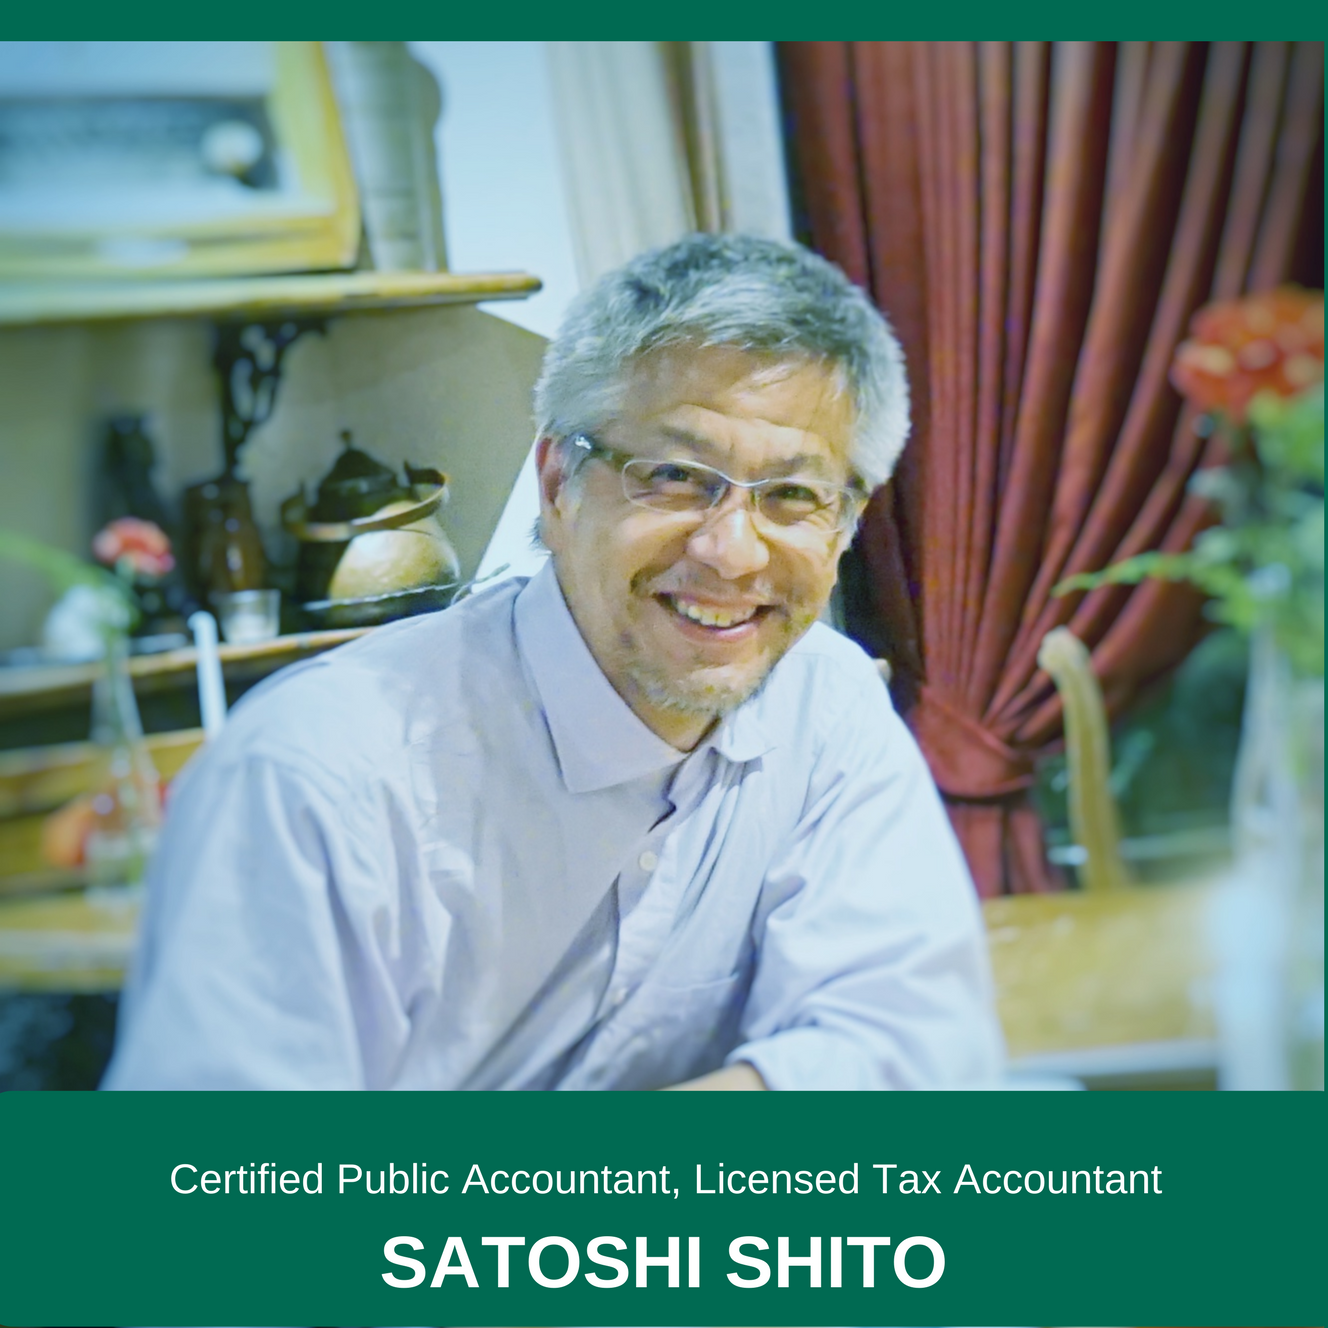
\includegraphics[width=35mm]{shirokanecpa.png}
%\end{wrapfigure}
\end{minipage}

%\vspace{-55mm}    %横書き用
\vspace{-35mm}
\section{My Profile}

\subsection{Personal Information}

\begin{table}[h]
%\begin{spacing}{0.9}
  \begin{tabular}{lll}
Name & {\sffamily \bfseries SATOHSI SHITO} & \\
Professional & \multicolumn{2}{l}{Certified Public Accountant, \textit{1999 (No. 020888)}} \\
\ licenses       & \multicolumn{2}{l}{Certified Tax Accountant, \textit{2013 (No. 127096)}} \\
Affiliation  & \multicolumn{2}{l}{Tokyo Tax Accountant Agency,} \\
 & \multicolumn{2}{l}{Tax Support committee at Shinagawa} \\
         & \multicolumn{2}{l}{Japan CPA Tax committee} \\
         & \multicolumn{2}{l}{Certified Support Agencies for Business Innovation} \\

\includegraphics[width=4mm]{phone.png} & {\sffamily \bfseries +81 80-1257-5877} & \\

\includegraphics[width=4mm]{mail.png} & {\sffamily \bfseries satoshi.shito@shirokanecpafirm.com} & \\

\includegraphics[width=4mm]{website.png} & \multicolumn{2}{l}{\href{https://www.shirokanecpa.com/}{ https://www.shirokanecpa.com/}} \\
 %           & \multicolumn{2}{l}{\href{https://www.shirokanecpafirm.com/}{Jp) https://www.shirokanecpafirm.com/}} \\

\includegraphics[width=4mm]{linkedin.png} & \multicolumn{2}{l}{https://www.linkedin.com/in/satoshishito/} \\    

\includegraphics[width=4mm]{facebook.png} & \multicolumn{2}{l}{Jp)https://www.facebook.com/shirokanecpafirmjp/} \\
            & \multicolumn{2}{l}{En) https://www.facebook.com/Shirokanecpafirm/} \\   
  \end{tabular}
%\end{spacing}
\end{table}

\subsection{Mission}
To navigate entrepreneurs, and  small and med-sized business with my professional skill and to bridge between foreign nationals and Japan business, wishing all of us keep growing to the future. 

%\subsection{Value}
%\subsubsection{Make Your Fixed Expense Minimized}
%On an early phase, your business might not be stable, and might not have enough revenue. Under such situation, if you had not small fixed expense, that could be a risk on your business.

%Accordingly, I believe that it would be good for you to start your business with small initial investment, that also could make your fixed expense small.

%I could suggest you to use cloud-based services, that could make you expense less than hiring an administrative employee. Besides, my services could help your administration work, like keeping your accounting book and filing some applications to the tax office.

%\subsubsection{Tax Scheme}
%\paragraph{Tax Rate}
%If you  had not spent many days on your business, your busness form on tax would be a solo-proprietor, that is a self-employed. Then, you are subject to individual income tax in Japan. If you had your company like K.K., you have to file a tax return on corporate income tax.

%The tax rate is different between individuals and companies. Therefore, if your income as a solo-proprietor is large enough, it would be better for your business to be run by a company.

%\paragraph{Consumption Tax}
%When you have more than JPY 10 million taxable revenue, you are taxed after 2 years. Consumption tax obligation is determined by this JPY 10 million taxable revenue rule. This is also applied to the company that has capital amount less than JPY 10 million.
% 未完成

%\paragraph{Deduction}

%\subsubsection{Meet Your Budget}


\subsection{Background}

\subsection*{\normalsize \itshape \bfseries Jan 2014-Present}
{\bfseries \itshape Supporting SME by Consulting Business and Tax} \\
\begin{itemize}
\begin{spacing}{0.6}
  \item Established Shirokane CPA Firm in 2014.
  \item Working on consulting IT\& Design company, Investment Advisory Company.
  \item Working on Tax filing of a non-profit entity governed by SHINAGAWA-ku
%  \item Consulted Kidslox Ltd. (U.K. company) to sale the app in Japan.
  \item Supporting incorporation of K.K., G.K., ISH, especially for foreign nationals and foreign companies.
\end{spacing}
\end{itemize}

\subsection*{\normalsize \itshape \bfseries Sep 2011-Dec 2013}
{\bfseries \itshape Cross Border Management and Cooperation}
\begin{itemize}
\begin{spacing}{0.6}
  \item Worked on Japan Microsoft K.K.'s statutory audit as an audit in-charge.
  \item Worked on SBI Holding, Inc.'s IPO consulting to Hong Kong Stock Exchange as an in-charge of a Japan project team, cooperating with Hong Kong Deloitte team.
  \item Experienced one divestiture of Canadian company and one starting up company in Shanghai on Minit Asia Pacific K.K.'s statutory audit I had worked as an audit in-charge.
\end{spacing}
\end{itemize}

\subsection*{\normalsize \itshape \bfseries Jun 2004-Sep 2011}
{\bfseries \itshape Building a Listing Company through IPO Consulting} \\
Worked on Loan Star group as an in-charge of IPO consulting team.

{\bfseries \itshape Internal Control Consulting} \\
Worked on PGM Holdings K.K. as an in-charge of the consulting team to prepare with Internal Control Audit (called Japan-SOX).

{\bfseries \itshape Group Audit and IPO consulting}
\begin{itemize}
\begin{spacing}{0.6}
  \item Worked on PGM Holdings K.K. as an in-charge of the audit team.
  \item Worked on preliminary surveys for IPO to Goldman Sachs. 
\end{spacing}
\end{itemize}

\subsection*{\normalsize \itshape \bfseries Oct 1999-Jun 2004}
{\bfseries \itshape Verious Statutory Audit} \\
Worked on mainly statutory audit of some industries like, banks, lease companies, manufacturing companies, construction companies, educational corporations, wholesale and logistic companies, and retail companies. Besides, experienced preliminary surveys for IPO, IPO consulting, and due diligence for acquisition.

%\subsection{Personal Activities}

%{\bfseries \itshape Down-hill Skiing (off-piste):} \\
%From the top of following mountains, \\
%Mt. Fuji (\textit{the highest in Japan, 2012, 2013, and 2014}) \\
%Okuhodaka (\textit{3rd highest in Japan, 2013}) \\
%Harinoki (\textit{2,821m, 2008, 2009}), Tanigawa (\textit{1,977m, 2012-}) \\

%{\bfseries \itshape Traveling:} \\
%California and Oregon, U.S.  (\textit{1991})\\
%Austria (\textit{1998}), Australia (\textit{1998}) \\
%Poland and Estonia (\textit{2015}) \\
%Croatia, Bosnia and Herzegovina, and Montenegro (\textit{2016}) \\
%Domestic area \\
             
%{\bfseries \itshape Scuba Diving:} \\       
%Certification of Advanced Open Water Diver. Experience of \\
%TAKA Dive's 5days cruise  (\textit{1999}) and two 4days diving trips with catamaran yacht at Okinawa, Japan (\textit{2008, 2000}). \\
